\documentclass{article}
\usepackage[T1]{fontenc}
\usepackage[utf8]{inputenc}
\usepackage[table,xcdraw]{xcolor}
\usepackage{graphicx}
\usepackage{hyperref}
\usepackage{xcolor}

\definecolor{linkcolor}{HTML}{FF1493} 
\definecolor{urlcolor}{HTML}{1E90FF} 
 
\hypersetup{pdfstartview=FitH,  linkcolor=linkcolor,urlcolor=urlcolor, colorlinks=true}
\title{Hobbies}
\author{Vadzim Shyshko }
\date{8 January 2020}

\begin{document}

\maketitle

\tableofcontents
\listoffigures
\listoftables
\newpage
\section{Information about hobbies}
\subsection{List of popular Hobbies}

\begin{enumerate}
\item Blogging,
\item Collecting,
\item Dance,
\item Fashion,
\item Fishing,
\item Caving,
\item Photography.
\end{enumerate}

\subsection{Role of hobbies in our life}
Having a hobby that we enjoy brings us joy and enriches our lives. It gives us something fun to do during our leisure time and affords us the opportunity to learn new skills. We are very fortunate to have so many different options out there today. In fact, there are entire websites devoted to hobbies and interests.

The best way to cultivate a new hobby is to try something new. The world is full of wonderful, exciting activities that we can explore and adopt as our own. Of course, all of us are unique and, therefore, our interests and hobbies vary. But once we find a hobby that we truly enjoy and are passionate about, we become hooked. It becomes part of our lives and captivates us in a very personal way.

\section{My hobby - Photography}   
\href{https://en.wikipedia.org/wiki/Photography}{Cllick}

\subsection{What is photography?}
Photography is the art, application and practice of creating durable images by recording light or other electromagnetic radiation, either electronically by means of an image sensor, or chemically by means of a light-sensitive material such as photographic film. It is employed in many fields of science, manufacturing (e.g., photolithography), and business, as well as its more direct uses for art, film and video production, recreational purposes, hobby, and mass communication.

\newpage
\subsection{Social and cultural implications}

\begin{itemize}
\item There are many ongoing questions about different aspects of photography. In her On Photography (1977), Susan Sontag dismisses the objectivity of photography. This is a highly debated subject within the photographic community.[61] Sontag argues, "To photograph is to appropriate the thing photographed. It means putting one's self into a certain relation to the world that feels like knowledge, and therefore like power."[62] Photographers decide what to take a photo of, what elements to exclude and what angle to frame the photo, and these factors may reflect a particular socio-historical context. Along these lines, it can be argued that photography is a subjective form of representation.

Modern photography has raised a number of concerns on its effect on society. In Alfred Hitchcock's Rear Window (1954), the camera is presented as promoting voyeurism. 'Although the camera is an observation station, the act of photographing is more than passive observing.
\item The camera doesn't rape or even possess, though it may presume, intrude, trespass, distort, exploit, and, at the farthest reach of metaphor, assassinate – all activities that, unlike the sexual push and shove, can be conducted from a distance, and with some detachment.
\end{itemize}

\begin{table}[]
\begin{tabular}{|c|c|c|c|}
\hline
\multicolumn{4}{|c|}{Types of photography}                                                             \\
\hline
Amateur                                                                                             
& Art   
& Photojournalism                                                                                   
& Science and forensics                                                                                \\ \hline
\begin{tabular}[c]{@{}c@{}}An amateur \\ photographer \\ is one who \\ practices \\ photography as a \\ hobby/passion \\ and not necessarily \\ for profit. Good\\  pictures \\ can now be \\ taken with \\ a cell phone \\ which is a\\  key tool for\\  making \\ photography more \\ accessible to \\ everyone.\end{tabular} & \begin{tabular}[c]{@{}c@{}}During the 20th \\ century, both \\ fine art photography \\ and documentary \\ photography became \\ accepted by the \\ English-speaking \\ art world and the \\ gallery system. In \\ the United States,\\ a handful of \\ photographers, \\ including Alfred Stieglitz, \\ Edward Steichen, \\ John Szarkowski, \\ F. Holland Day, and \\ Edward Weston, \\ spent their lives \\ advocating for \\ photography as a fine art.\end{tabular} & \begin{tabular}[c]{@{}c@{}}Photojournalism is \\ a particular form of \\ photography (the \\ collecting, editing,\\ and presenting of news \\ material for \\ publication or broadcast)\\ that employs images\\  in order to tell a \\ news story. It is now \\ usually understood\\  to refer only to still \\ images, but in some \\ cases the term also \\ refers to video used \\ in broadcast journalism.\end{tabular} & \begin{tabular}[c]{@{}c@{}}The camera has \\ a long and \\ distinguished history \\ as a means of \\ recording scientific \\ phenomena from the \\ first use by Daguerre \\ and Fox-Talbot, such \\ as astronomical events \\ (eclipses for example), \\ small creatures and \\ plants when the \\ camera \\ was attached to the \\ eyepiece of \\ microscopes \\ (in photomicroscopy)\\ andfor macro\\ photography \\ of larger specimens.\end{tabular} \\ \hline
\end{tabular}
\end{table}

\begin{figure}[ht]
\begin{center}
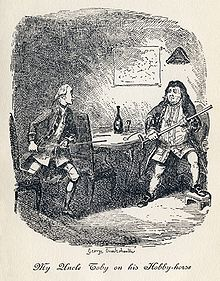
\includegraphics[width=7cm]{hobby.jpg}
\caption{The origin of the word hobby in Tristram Shandy,} {a r' "hobby-horses", or particular obsessions}
\label{rys_model}
\end{center}
\end{figure}

\subsection{Math formulas}
\begin{center}
Formula of a good life\\
a-moment in the life when you was happy\\
b-moment in the life when you was unhappy
\end{center}
$$\int^a_b \frac{1}{3}x^3+\frac{1}{\sqrt{x}}$$
\begin{center}
Formula usual life
\end{center}
\begin{equation}
\sum_{i=1}^{n} \qquad \int_{0}^{\frac{\pi}{2}} \qquad x^ {c+d}={a+b}\\
\end{equation}

\newpage
\begin{thebibliography}{9}
\bibitem{Book 1}
The Phrase Finder,
\emph{ Gary Martin }
2012.
\href{https://www.loc.gov/item/lcwaN0004219/}{Click}
 
\bibitem{Book 2}
Hobbies: leisure and the Culture of Work in America,
\emph{ Gelber S M }
1999.
\end{thebibliography}

\end{document}

